\subsection{Bayesian Inference}

For each output variable, the user specifies an observed value (from
physical experiments) with the associated uncertainties (in the form of
standard deviation), if applicable. Whether standard inference or
SolventFit is selected, the tool will launch a Markov Chain Monte Carlo (MCMC)
algorithm to compute the posterior distributions of the uncertain input
parameters. These input posterior distributions represent a refined
hypothesis about the input uncertainties in light of what was previously
known (in the form of input prior distributions) and what was observed
currently (in the form of noisy outputs).

\begin{enumerate}
\item{Load the file ``lptau5k\_10inputs\_4outputs.filtered'' from the examples\bs UQ folder.}
\item{Click \bu{Analyze} for the current ensemble and a new dialog box displays (Figure \ref{fig:uqt_analysis_infer}).
%%% INSERT: Analysis Screen, Bayesian Inference Selection
\begin{figure}[H]
\centering 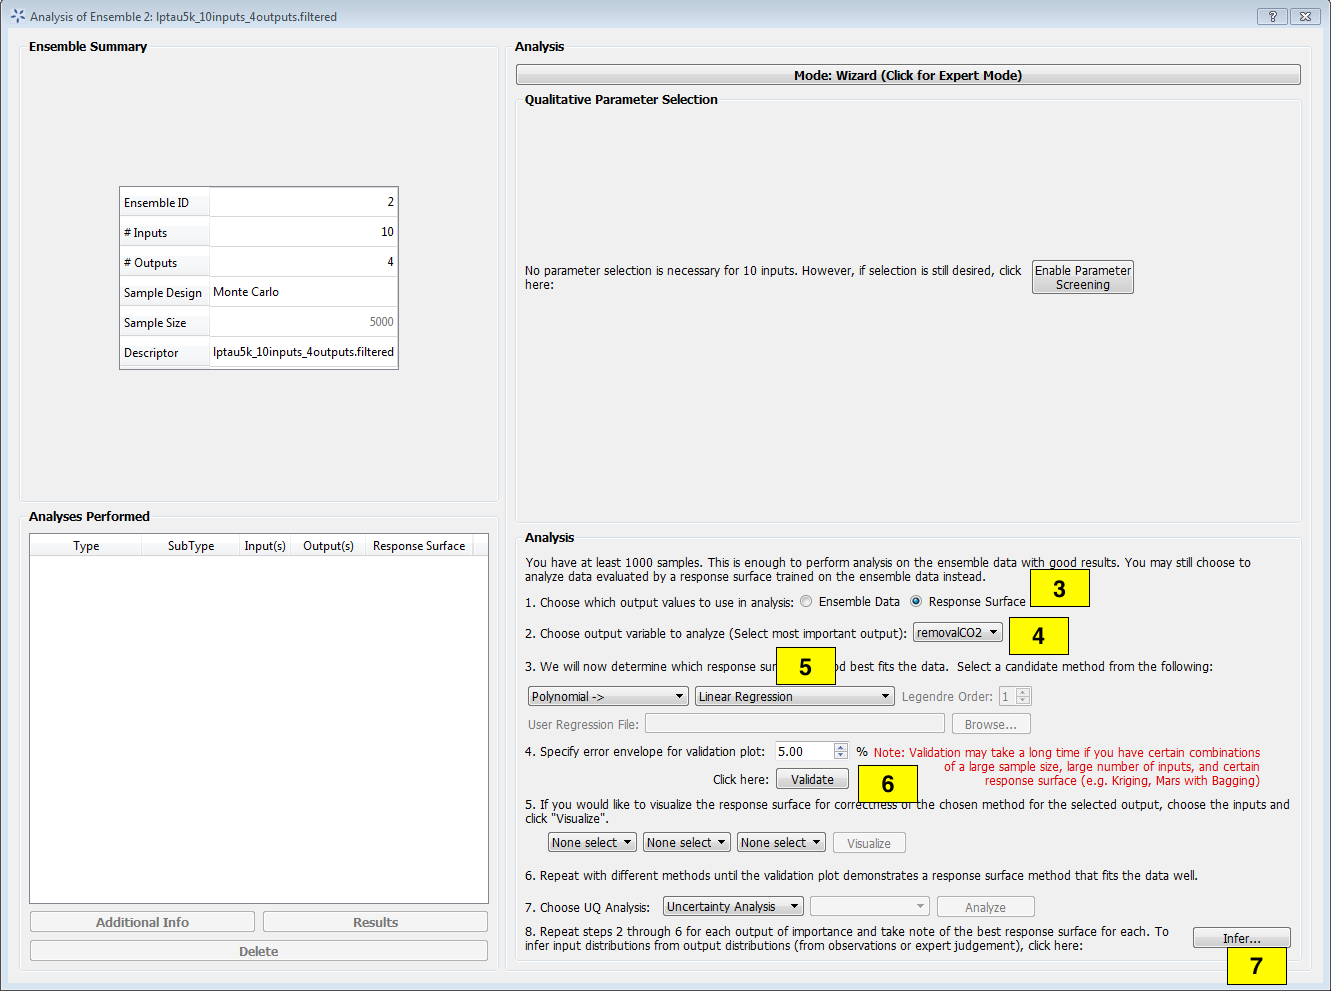
\includegraphics[width=6.5in,height=4in,keepaspectratio]{Chapt_uq/figs/tutorial/29_InfSelection2}
\caption{Analysis Dialog, Bayesian Inference}
\label{fig:uqt_analysis_infer}
\end{figure}
}
\item{Select ``Response Surface'' in the ``Analysis'' section.}
\item{Select ``Output variable to analyze'' to be ``removalCO2.''}
\item{Select ``Linear Regression'' as the response surface.}
\item{Insert 5.00 as the error envelope for the validation plot. Click \bu{Validate}. The GUI allows the user to proceed with Bayesian
  inference after one input has been validated; however, the user may want
  to validate all outputs since they are all used in the inference.}
\item{Once validation is completed, click \bu{Infer} at the lower right
  corner, which displays a new dialog box (Figure \ref{fig:uqt_infer}).}
\item{In the \bu{Output Settings} table (on the left), select the second, third, and fourth outputs as the observed outputs.
  The user
  can experiment with using different response surface models (for example,
  linear polynomials) to approximate the mapping from inputs to each of the
  outputs. }
\item{In the \bu{Input Settings} table (on the right), 
  designate input types (variable, design, or fixed) and if necessary,
  switch to Expert Mode to revise the prior distribution on the input parameters.
  The prior distribution represents knowledge that the user possesses about
  the inputs before observational data (from experiments) has been
  incorporated into this knowledge. If the user does not have any updated
  knowledge about the simulation ensemble, it is OK to leave the table as is.}  
\item{In the \bu{Observations} table (in the middle), select the number of
  experiments from which the user can get observational data. In essence, if the user
  has $N$ observations, then $N$ should be set as the number of
  experiments. The table will then populate columns for design inputs (if
  any) and observed outputs. Currently, only normal distribution is
  supported as the noise model for observations. Enter the mean and standard deviation for each of these observations.
  For convenience,
  the mean and standard deviation values are prepopulated with the results from uncertainty analysis. These
  values have been provided as a sanity check for the user, in case the
  observation for a particular output is way out of range from these
  distributions.
%%% INSERT: Bayesian Inference Screen
\begin{figure}[H]
\centering 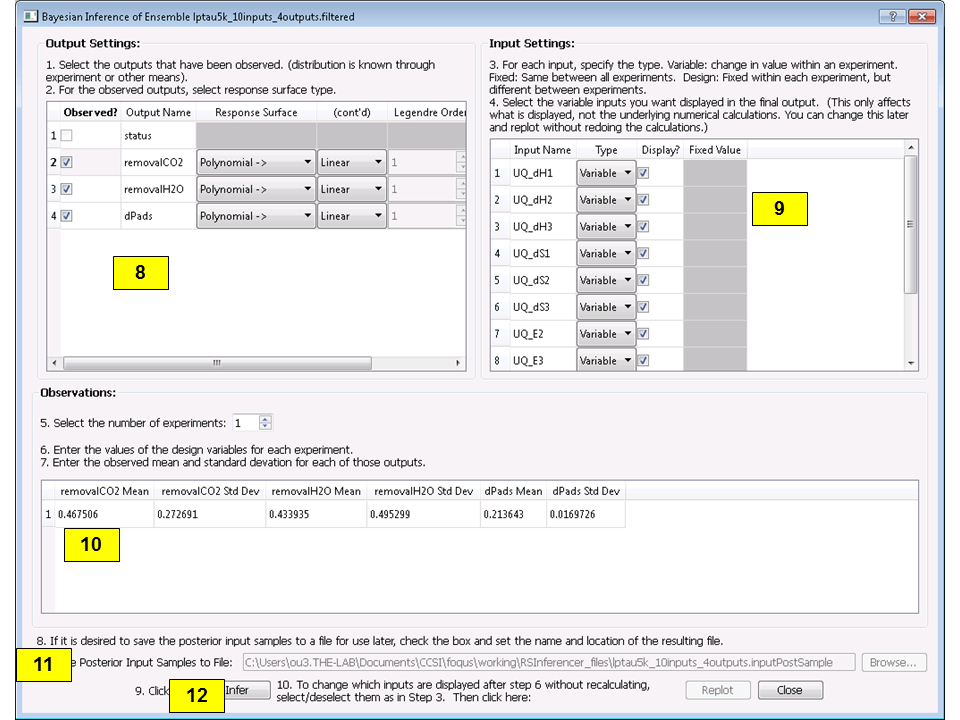
\includegraphics[width=6.5in,height=4in,keepaspectratio]{Chapt_uq/figs/tutorial/30_InfScreen2}
\caption{Bayesian Inference Dialog for Standard Inference}
\label{fig:uqt_infer}
\end{figure}
}
\item{To save an input sample drawn from the posterior distribution,
  select the \textbf{\underline{Save Posterior Input Samples to File}} checkbox and
  select a location and file name to store the sample.}
\item{Click \bu{Infer} to start the analysis. Inference can take a long
  time; thus, a stop feature has been implemented. Once inference starts,
  the \textbf{\underline{Infer}} button changes to \textbf{\underline{Stop}}. To stop inference
  calculations, click \textbf{\underline{Stop}} which changes the button back to \textbf{\underline{Infer}},
  allowing the user to restart the calculations from scratch. If inference
  is allowed to run its course, its results are interpolated to produce
  heat maps (off-diagonal subplots in Figure \ref{fig:uqt_infer_results}) for
  visualization. This interpolation step can take a few minutes and while
  it is running, \textbf{\underline{Infer}} is disabled.}
\end{enumerate}

%%% INSERT: Bayesian Inference Results
\begin{figure}[H]
\centering
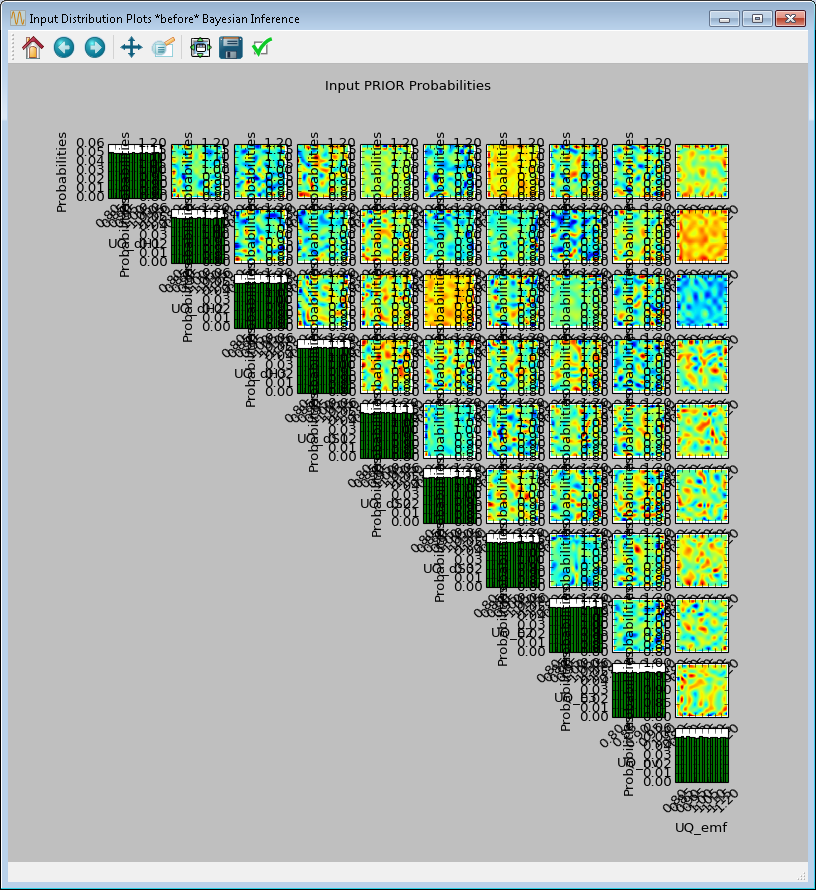
\includegraphics[width=6.5in,height=4in,keepaspectratio]{Chapt_uq/figs/tutorial/31a_InfPriorResults}
\centering
\includegraphics[width=6.5in,height=4in,keepaspectratio]{Chapt_uq/figs/tutorial/31_InfResults}
\caption{Bayesian Inference Results}
\label{fig:uqt_infer_results}
\end{figure}

Once the inference and interpolation steps are complete, two windows will
be displayed: a multi-plot figure of the prior distributions and another
multi-plot figure of the posterior distributions. 
If the user has selected the \textbf{\underline{Save Posterior Input Samples to File}} checkbox,
then a sample file will also be written to the designated file location.

In the resulting prior and posterior plots 
(Figure \ref{fig:uqt_infer_results}), the univariate
input distributions are displayed as histograms on the
diagonal. The bivariate input distributions (between pairs of inputs)
are displayed as heat maps in the off-diagonal subplots. On these heat
maps, the regions in red reflect the input space with higher probability. 
In the posterior plots, the red regions represent inputs that are more
likely to have generated the specified observations on the outputs. By
comparing the prior and the posterior figures, the user can see the ''before''
and ''after'' impact of inference on our knowledge of the input
uncertainty.

To zoom in on any one of the subplots, left-click; to zoom out, right-click.
To display a subset of these subplots, clear the checkbox for the inputs to be omitted
(from the first column of the Input Prior Table) and click \textbf{\underline{Replot}}
(Figure \ref{fig:uqt_infer_replot_results}). 

%%% INSERT: Bayesian Inference Replot Results
\begin{figure}[H]
\centering
\includegraphics[width=6.5in,height=4in,keepaspectratio]{Chapt_uq/figs/tutorial/32a_InfPriorReplotResults}
\centering
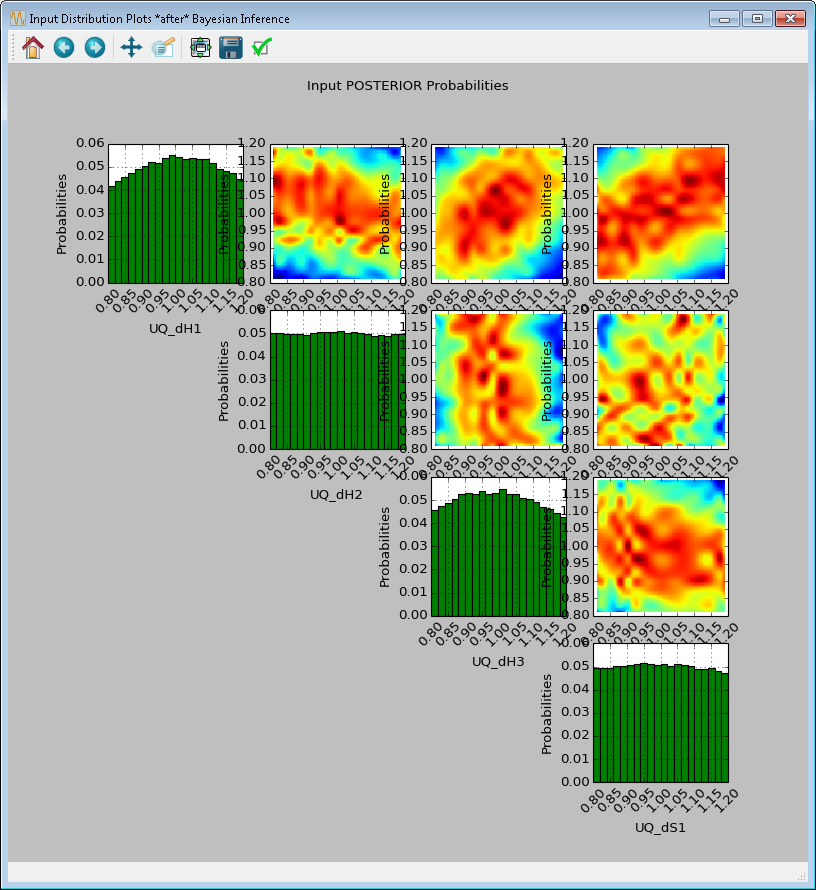
\includegraphics[width=6.5in,height=4in,keepaspectratio]{Chapt_uq/figs/tutorial/32_InfReplotResults}
\caption{Bayesian Inference Replot Results}
\label{fig:uqt_infer_replot_results}
\end{figure}
